\documentclass{article}\usepackage{graphicx, color}
%% maxwidth is the original width if it is less than linewidth
%% otherwise use linewidth (to make sure the graphics do not exceed the margin)
\makeatletter
\def\maxwidth{ %
  \ifdim\Gin@nat@width>\linewidth
    \linewidth
  \else
    \Gin@nat@width
  \fi
}
\makeatother

\IfFileExists{upquote.sty}{\usepackage{upquote}}{}
\definecolor{fgcolor}{rgb}{0.2, 0.2, 0.2}
\newcommand{\hlnumber}[1]{\textcolor[rgb]{0,0,0}{#1}}%
\newcommand{\hlfunctioncall}[1]{\textcolor[rgb]{0.501960784313725,0,0.329411764705882}{\textbf{#1}}}%
\newcommand{\hlstring}[1]{\textcolor[rgb]{0.6,0.6,1}{#1}}%
\newcommand{\hlkeyword}[1]{\textcolor[rgb]{0,0,0}{\textbf{#1}}}%
\newcommand{\hlargument}[1]{\textcolor[rgb]{0.690196078431373,0.250980392156863,0.0196078431372549}{#1}}%
\newcommand{\hlcomment}[1]{\textcolor[rgb]{0.180392156862745,0.6,0.341176470588235}{#1}}%
\newcommand{\hlroxygencomment}[1]{\textcolor[rgb]{0.43921568627451,0.47843137254902,0.701960784313725}{#1}}%
\newcommand{\hlformalargs}[1]{\textcolor[rgb]{0.690196078431373,0.250980392156863,0.0196078431372549}{#1}}%
\newcommand{\hleqformalargs}[1]{\textcolor[rgb]{0.690196078431373,0.250980392156863,0.0196078431372549}{#1}}%
\newcommand{\hlassignement}[1]{\textcolor[rgb]{0,0,0}{\textbf{#1}}}%
\newcommand{\hlpackage}[1]{\textcolor[rgb]{0.588235294117647,0.709803921568627,0.145098039215686}{#1}}%
\newcommand{\hlslot}[1]{\textit{#1}}%
\newcommand{\hlsymbol}[1]{\textcolor[rgb]{0,0,0}{#1}}%
\newcommand{\hlprompt}[1]{\textcolor[rgb]{0.2,0.2,0.2}{#1}}%

\usepackage{framed}
\makeatletter
\newenvironment{kframe}{%
 \def\at@end@of@kframe{}%
 \ifinner\ifhmode%
  \def\at@end@of@kframe{\end{minipage}}%
  \begin{minipage}{\columnwidth}%
 \fi\fi%
 \def\FrameCommand##1{\hskip\@totalleftmargin \hskip-\fboxsep
 \colorbox{shadecolor}{##1}\hskip-\fboxsep
     % There is no \\@totalrightmargin, so:
     \hskip-\linewidth \hskip-\@totalleftmargin \hskip\columnwidth}%
 \MakeFramed {\advance\hsize-\width
   \@totalleftmargin\z@ \linewidth\hsize
   \@setminipage}}%
 {\par\unskip\endMakeFramed%
 \at@end@of@kframe}
\makeatother

\definecolor{shadecolor}{rgb}{.97, .97, .97}
\definecolor{messagecolor}{rgb}{0, 0, 0}
\definecolor{warningcolor}{rgb}{1, 0, 1}
\definecolor{errorcolor}{rgb}{1, 0, 0}
\newenvironment{knitrout}{}{} % an empty environment to be redefined in TeX

\usepackage{alltt}

\begin{document}

\section{Introduction}
\subsection{Synopsis}
Package {\tt cgmisc} contains miscellaneous functions, hopefully useful for extending genome-wide association study (GWAS) analyses. 

\subsection{Getting help}
Like every other R function, the functions provided in this package are documented in the standard R-help (Rd) format and can be easily accessed by issuing {\tt help()} or its shorter version, {\tt ?} function. For instance, if you want to get more information on how to use the {\tt clump.markers()} function, type either {\tt help(clumpmarkers)} or {\tt ?clump.markers} and press return/enter. To see this document from within R you type {\tt vignette('cgmisc')}. 

\subsection{Purpose of this document}
This document aims at presenting how to use functions provided in this package in a typical GWAS data analyses workflow. It is, however, not pretending to be a GWAS tutorial as such.

\subsection{Conventions}
\begin{itemize}
  \item{All R commands are written in terminal type: {\tt myfun(foo=T, bar=54)}}
  \item{In the above example: {\tt myfun} is a \textit{function} and both {\tt foo} and {\tt bar} are its \textit{arguments}}
\end{itemize}

\section{Working with {\tt cgmisc}}
\subsection{Installation}
In order to install {\tt cgmisc}, you either use one of the R GUIs (native R GUI, RStudio etc.) or type the following command:
\begin{knitrout}
\definecolor{shadecolor}{rgb}{0.969, 0.969, 0.969}\color{fgcolor}\begin{kframe}
\begin{alltt}
\hlfunctioncall{install.packages}(\hlstring{"cgmisc"}, repos = \hlstring{""})
\end{alltt}
\end{kframe}
\end{knitrout}

\noindent Functions in the {\tt cgmisc} package often complement or use {\tt GenABEL} \ref{aulchenko} package functions and data structures. {\tt GenABEL} is an excellent and widely-used R package for performing genome-wide association studies and much more... Therefore {\tt GenABEL} will be loaded automagically when loading {\tt cgmisc}. If for some mysterious reason this does not happen, you can install and load {\tt GenABEL} by typing:
\begin{knitrout}
\definecolor{shadecolor}{rgb}{0.969, 0.969, 0.969}\color{fgcolor}\begin{kframe}
\begin{alltt}
\hlfunctioncall{install.packages}(\hlstring{"GenABEL"})
\hlfunctioncall{require}(\hlstring{"GenABEL"})
\end{alltt}
\end{kframe}
\end{knitrout}

\noindent You load {\tt cgmisc} package in exactly the same way (both {\tt require} and {\tt library} will do):
\begin{knitrout}
\definecolor{shadecolor}{rgb}{0.969, 0.969, 0.969}\color{fgcolor}\begin{kframe}
\begin{alltt}
\hlfunctioncall{require}(\hlstring{"cgmisc"})
\end{alltt}


{\ttfamily\noindent\itshape\color{messagecolor}{\#\# Loading required package: cgmisc}}

{\ttfamily\noindent\itshape\color{messagecolor}{\#\# Loading required package: GenABEL}}

{\ttfamily\noindent\itshape\color{messagecolor}{\#\# Loading required package: MASS}}

{\ttfamily\noindent\itshape\color{messagecolor}{\#\# GenABEL v. 1.7-4 (February 22, 2013) loaded}}\begin{alltt}
\hlfunctioncall{library}(\hlstring{"cgmisc"})  # Alternative to require
\end{alltt}
\end{kframe}
\end{knitrout}

\noindent After having loaded the package it is time to load some data:
\begin{knitrout}
\definecolor{shadecolor}{rgb}{0.969, 0.969, 0.969}\color{fgcolor}\begin{kframe}
\begin{alltt}
\hlfunctioncall{data}(cgmiscdat1)
\end{alltt}
\end{kframe}
\end{knitrout}

\section{Using {\tt plot.Manhattan.LD} function}
The {\tt plot.Manhattan.LD} function allows you to visualize the LD pattern in a genome fragment on an enchanced Manhattan plot. You select one marker, typically the one with the strongest association to the analysed trait and all other markers in the region are coloured according to the degree of linkage disequilibrium with this index marker. You need to begin by running a standard GWAS analyses:
\begin{knitrout}
\definecolor{shadecolor}{rgb}{0.969, 0.969, 0.969}\color{fgcolor}\begin{kframe}
\begin{alltt}
\hlcomment{# Run association analyses}
an <- \hlfunctioncall{qtscore}(cad ~ sex, data = cgmiscdat1)
\end{alltt}


{\ttfamily\noindent\color{warningcolor}{\#\# Warning: binomial trait is analysed as gaussian}}

{\ttfamily\noindent\color{warningcolor}{\#\# Warning: 27 observations deleted due to missingness}}\begin{alltt}
\hlfunctioncall{plot}(an, pch = 19, cex = 0.5)  \hlcomment{# Plot standard Manhattan}
\end{alltt}
\end{kframe}
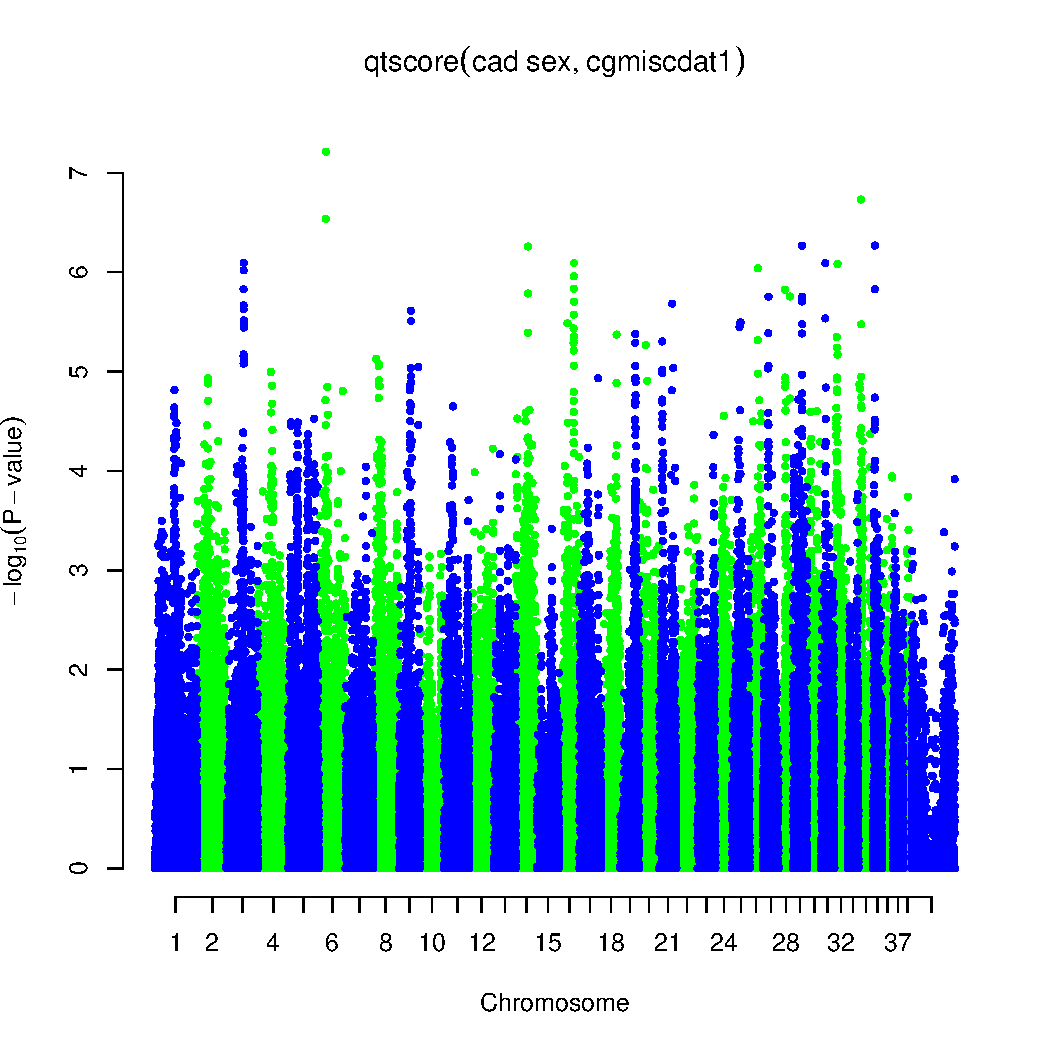
\includegraphics[width=\maxwidth]{figure/plot_Manhattan_LD} 

\end{knitrout}

Once this is done, you might be interested in checking the top associated marker. This can be done using the following call:
\begin{knitrout}
\definecolor{shadecolor}{rgb}{0.969, 0.969, 0.969}\color{fgcolor}\begin{kframe}
\begin{alltt}
\hlfunctioncall{summary}(an, top = 5)  \hlcomment{# List top 5 markers}
\end{alltt}
\begin{verbatim}
## Summary for top 5 results, sorted by P1df
##                 Chromosome Position Strand A1 A2   N    effB se_effB
## BICF2P453669             6 23340000      u  C  T 180 -0.2947 0.05443
## BICF2P1299812           34 10230234      u  G  A 180 -0.2729 0.05234
## BICF2P564616             6 23257649      u  C  T 180 -0.2621 0.05110
## BICF2G630770115         35  8408042      u  G  A 180 -0.3082 0.06150
## BICF2G630627595         29 29951256      u  G  A 180  0.2493 0.04975
##                 chi2.1df      P1df   effAB   effBB chi2.2df      P2df
## BICF2P453669       29.32 6.125e-08 -0.3111 -0.5754    29.40 4.123e-07
## BICF2P1299812      27.18 1.854e-07 -0.2806 -0.5447    27.19 1.245e-06
## BICF2P564616       26.31 2.902e-07 -0.2596 -0.5254    26.32 1.931e-06
## BICF2G630770115    25.12 5.395e-07 -0.2944 -0.6416    25.18 3.402e-06
## BICF2G630627595    25.11 5.416e-07  0.3391  0.4561    26.92 1.429e-06
##                     Pc1df
## BICF2P453669    0.0001053
## BICF2P1299812   0.0001888
## BICF2P564616    0.0002392
## BICF2G630770115 0.0003318
## BICF2G630627595 0.0003325
\end{verbatim}
\end{kframe}
\end{knitrout}

We can see that {\tt  ΒΙCF2P453669} on chromosome 6 (23.34Mb) is the strongest association. Now time to visualize a short fragment of chromosome 6, 1Mb downstream and 1Mb upstream of the top-associated marker.
\begin{knitrout}
\definecolor{shadecolor}{rgb}{0.969, 0.969, 0.969}\color{fgcolor}\begin{kframe}
\begin{alltt}
\hlfunctioncall{plot.manhattan.LD}(data = cgmiscdat1, gwas.result = an, chr = 6, region = \hlfunctioncall{c}(22340000, 
    24340000), index.snp = \hlstring{"BICF2P453669"}, p.value = 0.05, bonferroni = F, mafThreshold = 0.1)
\end{alltt}
\end{kframe}
\includegraphics[width=\maxwidth]{figure/plot_Manhattan_LD_3} 

\end{knitrout}

\end{document}
